\chapter{免疫防治}
\begin{framed}
\noindent\textbf{【知识体系】}
\begin{center}
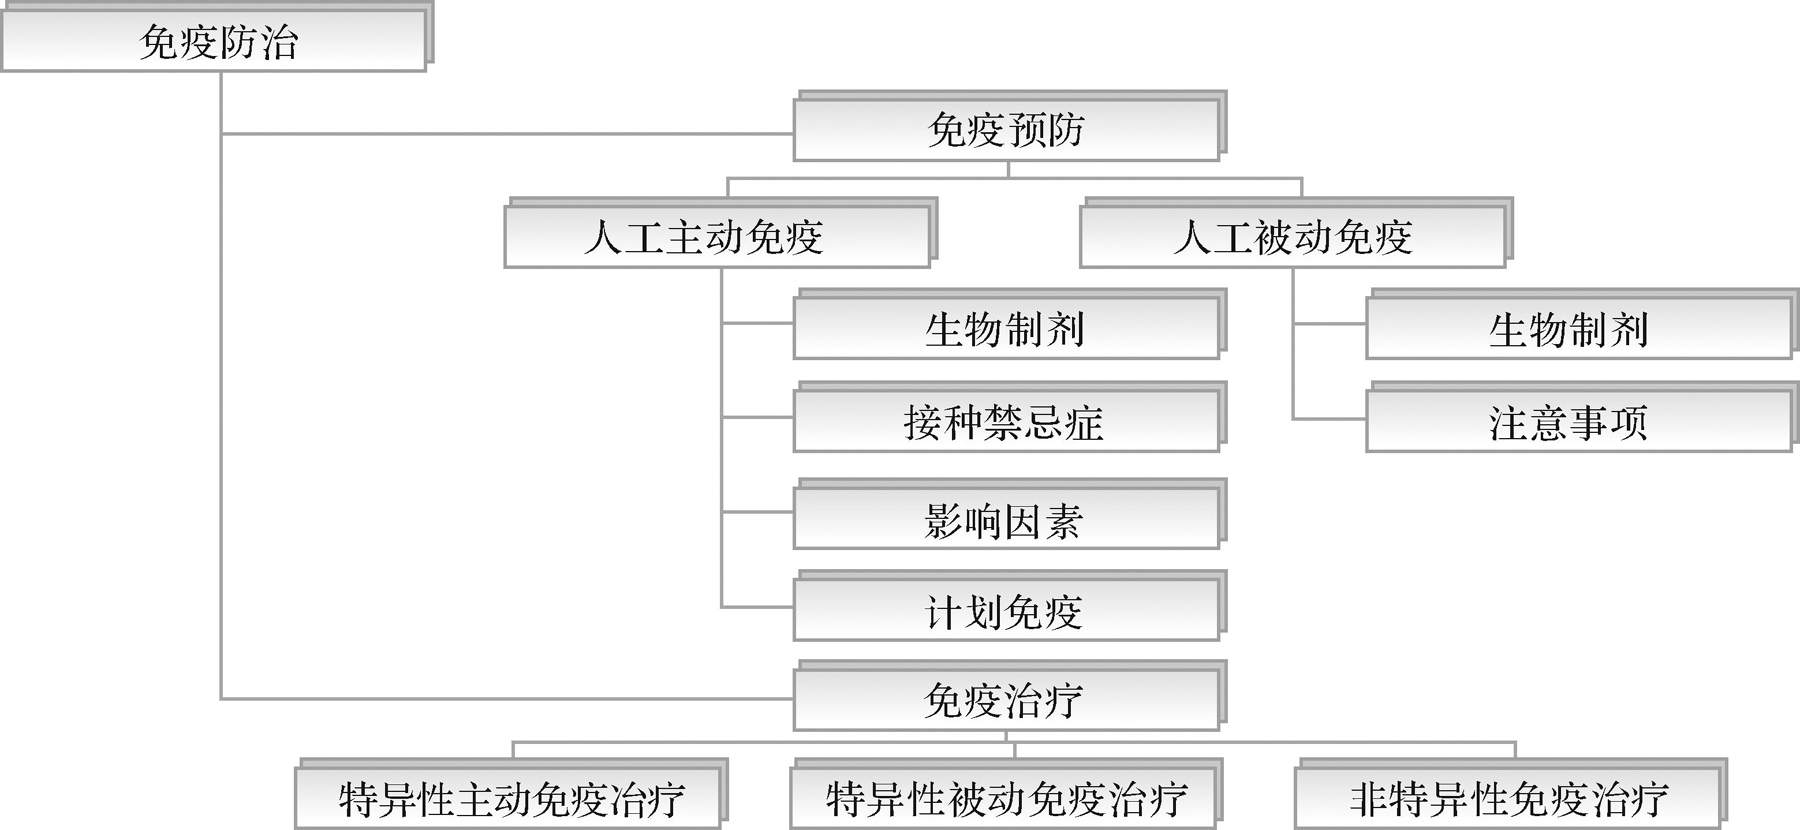
\includegraphics[width=.7\textwidth]{./images/Image00184.jpg}
\end{center}
\noindent\textbf{【课前思考】}

1.注射“乙肝疫苗、卡介苗、百白破三联疫苗”的目的是什么?机制?属于何种免疫?

2.注射“丙球、胎盘球蛋白、抗毒素、IL-2、IFN”的目的是什么?机制?属于何种免疫?

3.注射疫苗和注射丙球等制剂获得免疫力的方式各有什么特点?

4.请你举一个实例说明何时使用疫苗、何时使用丙球等制剂,并阐述理由及注意事项。

\noindent\textbf{【本章重点】}

1.人工主动免疫、人工被动免疫的特点、机理、影响因素;

2.特异性被动免疫治疗特点。

\noindent\textbf{【教学目标】}

1.熟悉免疫预防的种类;

2.人工主动免疫、人工被动免疫的特点、机理、影响因素。
\end{framed}

应用免疫制剂、免疫调节剂来建立、增强或抑制机体的免疫应答,调节免疫功能,达到预防和治疗疾病的目的称为免疫学防治。

\section{免疫预防}

免疫预防(immunoprophylaxis)是根据特异性免疫应答的原理,采用人工方法将抗原(疫苗、类毒素等)或抗体(免疫血清、丙种球蛋白等)制成各种制剂,接种于人体,使其产生特异性免疫力,达到预防某些疾病的目的。


\subsection{人工主动免疫}

人工主动免疫是通过接种疫苗使机体产生特异性免疫力(如对某种病原体的免疫力)的方法。用于人工主动免疫的、含有具有抗原性物质的生物制品被称为疫苗。

(一)人工主动免疫的疫苗

1.灭活疫苗

灭活疫苗又称死疫苗,是用经理化方法灭活的病原体制成的疫苗。伤寒、百日咳、霍乱、钩端螺旋体病、流感、狂犬病、乙型脑炎的病原体均已被制成了灭活疫苗。灭活疫苗进入人体后不能生长繁殖,对机体刺激时间短,要获得持久免疫力需多次重复接种。

2.减毒素疫苗

减毒活疫苗来源于“野生”的细菌和病毒,这些细菌或病毒的致病力通常在实验室通过传代培养而被削弱。活疫苗的免疫效果良好、持久,有减毒活疫苗恢复毒力,在接种后引发相应疾病的报道。免疫缺陷者和孕妇一般不宜接受活疫苗接种。目前应用的减毒活疫苗包括卡介苗、口服脊髓灰质炎疫苗、麻疹疫苗、风疹疫苗、腮腺炎疫苗、乙脑活疫苗、水痘疫苗等。

3.类毒素

细胞外毒素经甲醛处理后失去毒性,仍保留免疫原性,为类毒素。其中加适量磷酸铝和氢氧化铝即成吸附精制类毒素,其特点是:体内吸收慢,能长时间刺激机体,产生更高滴度抗体,增强免疫效果。接种类毒素可诱生机体产生相应外毒素的抗体,这种抗体被称为抗毒素,可中和外毒素的毒性。常用制剂的有破伤风类毒素和白喉类毒素等。

4.新型疫苗

(1)亚单位疫苗

亚单位疫苗是采用病原体能引起保护性免疫应答的成分制成的疫苗。例如,采用从乙型肝炎患者血浆中提取的乙型肝炎病毒表面抗原制成的乙型肝炎疫苗;采用从细菌提取的多糖成分制备的脑膜炎球菌、肺炎球菌、B型流感杆菌的多糖疫苗。

(2)基因工程疫苗

基因工程疫苗是采用重组DNA技术和细菌发酵或细胞培养技术生产的蛋白多肽类疫苗。如将乙型肝炎病毒表面抗原基因克隆入表达载体,再将此表达载体转入细菌或真核细胞,然后培养的细菌或细胞生产乙型肝炎病毒表面抗原,这种乙型肝炎病毒表面抗原就是一种基因工程疫苗。

(3)合成肽苗

用有效免疫原的氨基酸序列设计合成疫苗。合成肽分子小,免疫原性弱,常与脂质体交联诱导免疫应答。

(4)DNA苗

DNA苗是携带能引起保护性免疫反应的抗原基因的真核细胞表达质粒。这种质粒在直接接种机体后,抗原基因表达出相应的蛋白多肽,刺激机体的免疫系统发生免疫应答。该疫苗免疫效果好,持续时间长。

(5)转基因植物苗

将编码有效免疫原基因导入食用植物细胞基因中,免疫原在植物可食部位稳定表达,人类摄食达到接种目的。常用植物有番茄、马铃薯、香蕉。

理想疫苗应具备的条件:1)抗原高度纯化,无毒副作用;2)免疫力持久;3)免疫方法简单;4)可与其他抗原混合使用;5)价格便宜。

(二)接种禁忌症

1.既往诊断有明确过敏史儿童,一般不予接种

2.免疫缺陷者,应视为“绝对禁忌症”

3.正在发热者,应暂缓接种(除一般的呼吸道感染外,发热可能是某种疾病的先兆)

4.患有严重疾病者(急性传染病、重症慢性疾患、神经系统疾患和精神病)可暂缓接种,待痊愈后补种

5.各种疫苗还有不同禁忌症,应以说明书为准

(三)影响免疫效果的因素

1.疫苗使用方面

(1)免疫起始月龄提前,母传抗体干扰和个体免疫系统发育不成熟。

(2)接种剂量不足达不到有效免疫应答,超量则加重反应,甚至免疫麻痹或免疫抑制。

(3)次数:针次不足,影响免疫效果;针次过多,不必要的浪费,且增加反应。针次间隔过短或过长都可影响免疫效果。

(4)操作中忽略疫苗本身特性,如酒精未干接种麻疹或出针时用酒精棉球压针眼处,脊灰疫苗用热水送服等。

(5)疫苗贮运未按冷藏要求,使效价降低。

2.疫苗本身

(1)疫苗性质,活苗与灭活疫苗不同。

(2)疫苗菌毒种的抗原型,疫苗型别与流行的病原型别是否相符,有无交叉免疫。

(3)疫苗效价和纯度,所含有效抗原成分高,非抗原成分少。

(4)含有佐剂的疫苗效果优于不含佐剂的疫苗。

3.机体方面

(1)免疫功能不全或低下,或营养不良;

(2)患某些传染病后;

(3)或使用免疫抑制剂、免疫球蛋白被动免疫制剂等都会影响免疫效果。

(四)计划免疫

根据特定传染病疫情和人群免疫状况,有计划对儿童进行疫苗接种,以预防、控制、消灭传染病。我国目前的国家计划免疫是5苗防7病,即卡介苗、脊灰疫苗、百白破三联疫苗、麻疹疫苗和乙肝疫苗,主要预防结核病、脊髓灰质炎、百日咳、白喉、破伤风、麻疹和乙型肝炎(表\ref{tab11-1}、\ref{tab11-2})。

\begin{table}[htbp]
    \centering
    \caption{国家免疫规划疫苗的免疫程序}
    \label{tab11-1}
    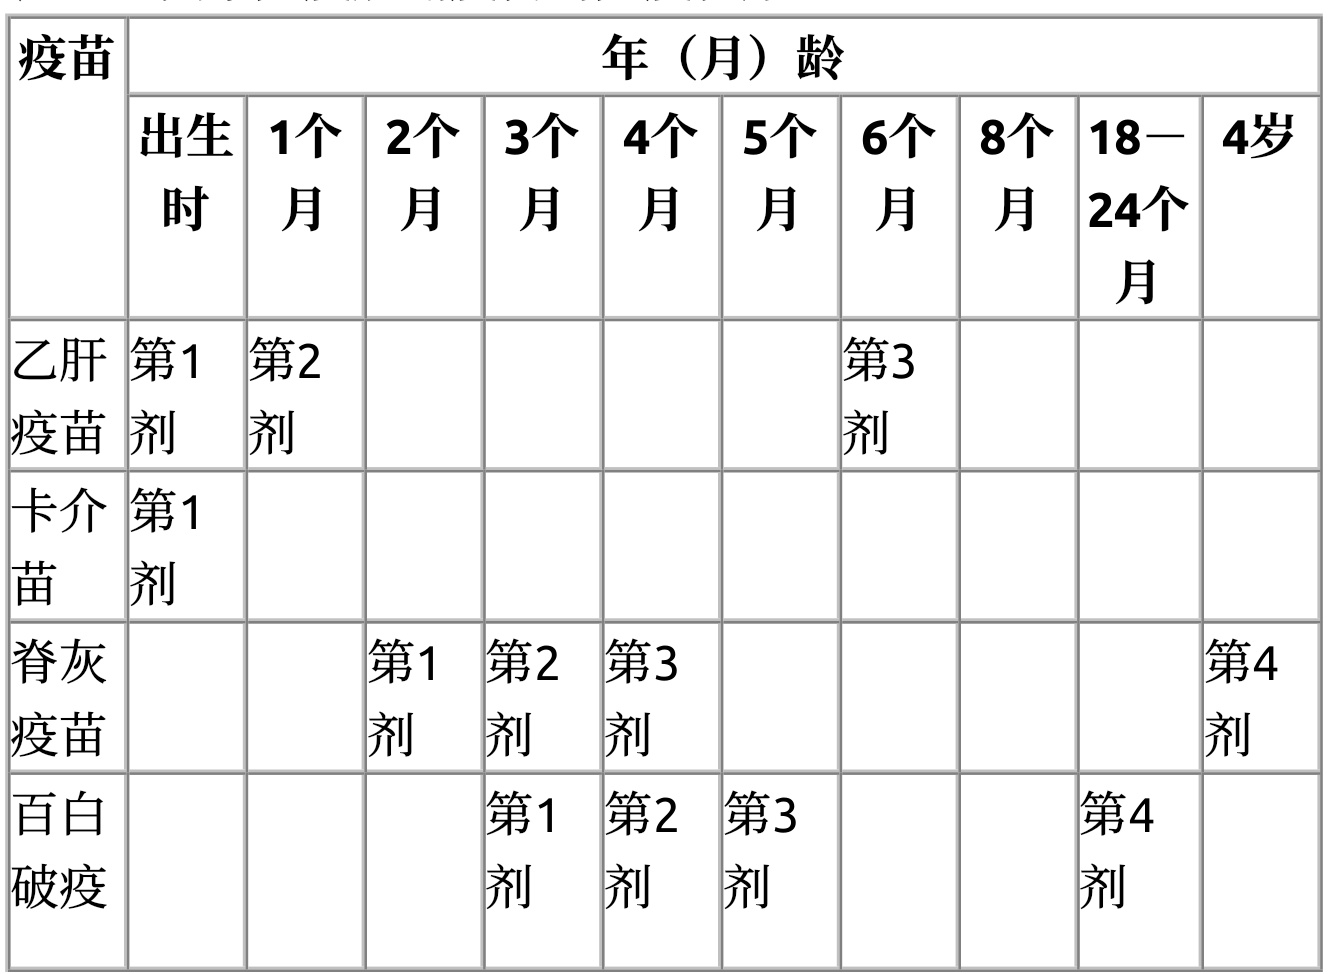
\includegraphics[width=.8\textwidth]{images/tab11-1.png}
\end{table}
\FloatBarrier
\begin{longtable}[]{p{3cm}p{4cm}p{4cm}p{4cm}}
    \caption{二类疫苗免疫程序}
    \label{tab11-2}\\
\toprule
疫苗名称 & 接种对象 & 免疫程序 & 预防疾病
\tabularnewline
\midrule
\endhead
甲肝疫苗 & 适用于1岁以上所有甲肝易感者 & 按“0、6 ”程序进行,即在注射第一针后六个月后加强免疫一针 & 甲型肝炎\\
乙肝疫苗 & 适用于所有乙肝易感者、尤其是儿童、青少年和乙肝病人、乙肝病毒携带者的密切接触者 & 按“0、1、6”程序进行,即在注射第一针后的1个月和6个月注射第二针和第三针 & 乙型肝炎\\
乙肝免疫球蛋白& (1)意外接触 HBV感染者的血液和体液后预防(2)新生儿,特别是乙肝病人或乙肝病毒携带者(HBs Ag和HBeAg阳性)母亲所生的婴儿 & (1)意外暴露预防:立即注射 HBIG200~400 IU,同时按“0,1,6”接种乙肝疫苗(2)母婴阻断。患乙肝、HBs Ag和HBeAg阳性母亲所生的婴儿出生12小时内注射100~200 IU,同时按“0,1,6”接种乙肝疫苗& 乙型肝炎\\
风疹疫苗& 青春期少女、育龄期妇女及12个月到14岁人群 & 对满8-18个月龄儿童初免、6岁加强;青春期少女、育龄期妇女注射一针 & 风疹、先天性风疹综合征\\
麻风腮疫苗/麻腮/麻风 & 青春期少女、育龄期妇女及12个月到15岁人群 & 对满8-18个月龄儿童初免、6岁加强;青春期少女、育龄期妇女注射一针 & 麻疹、风疹、腮腺炎\\
A+ C群流脑多糖体疫苗& 2岁以上所有易感人群& 对满6个月到18个月龄儿童初免两针 A群流脑疫苗;3、6岁加强免疫时可以使用A+ C群流脑疫苗,接种 A+C群流脑疫苗3年内避免重复接种& A群和C群流脑\\
A+C群流脑结合疫苗 & 6个月以上人群 & 6个月-2岁初免2针,间隔1个月;3、6岁儿童加强免疫各1针 & A群和C群流脑\\
无细胞百白破疫苗 & 3个月龄至6周岁的儿童 &新生儿出生后3足月接种第一针,连续接种3针,每针间隔时间最短不得少于28天;1岁半至2周岁时加强免疫1针& 白喉百日咳破伤风\\
流感疫苗 & 适用于成人和6个月龄以上儿童 &(1)成人和3岁以上儿童:接种1次,注射0.5毫升(2)6~36个月的儿童:接种1次,注射0.25毫升& 流行性感冒\\
狂犬疫苗 &特殊职业人群或宠物饲养者暴露前免疫凡被患有或疑患有狂犬病的动物咬伤、抓伤后均应接种& 按“0、7、28”程序进行,即在注射第一针后的7天和28天再注射第二针和第三针,共3针按“0、3、7、14、28”程序进行,即在伤者于0天(第1天,当天)、3天(第4天,依次类推)、7天、14天、28天各注射1针,共5针& 狂犬病\\
轮状病毒疫苗 & 2个月到3岁婴幼儿 & 2个月到3岁婴幼儿每年一次 & 婴幼儿A群轮状病毒引起的腹泻\\
B型流感嗜血杆菌疫苗 & 2个月71个月婴幼儿 &(1)2~6个月婴儿:连续接种3针,间隔1~2个月,18个月龄加强接种1针 (2)6~12个月婴儿:共两针,间隔1~2个月接种1针 (3)1~5岁儿童:接种1针& 由 B型流感嗜血杆菌引起的侵袭性疾病\\
水痘疫苗 & 12个月龄以上的水痘易感者 &(1)12个月龄~12岁无水痘感染史健康儿童接种1剂水痘疫苗(2)13岁及以上者接种2剂,间隔4~10周& 水痘\\
肺炎球菌多糖疫苗 & 2岁以上易感者尤其是老年人 &
2岁以上人群初免后,间隔5年左右加强1针 &由本疫苗所含荚膜菌型的肺炎球菌引起的肺炎球菌疾病\\
出血热疫苗 &肾综合征出血热疫区的居民及进入该地区的人员,主要对象为16~60岁的高危人群& 基础免疫2针,于0、14天各注射1次,6个月后加强免疫1针 &出血热\\
\bottomrule
\end{longtable}


\subsection{人工被动免疫}

给机体输入含有特异性抗体的免疫血清或细胞因子,把现成的免疫力转移给机体,以预防相应疾病的发生,称为人工被动免疫,这类生物制品称为“被动免疫制剂”。常用的人工被动免疫制剂有:抗毒素、丙种球蛋白及细胞因子等。人工被动免疫特点是:见效快,但维持时间短,仅2~3周,需要多次重复接种。所以人工被动免疫常用在治疗或紧急预防,在短时间内为免疫对象提供足够数量的抗体以得到针对一些感染的保护。

(一)抗毒素

1890年,Behring和Kitasato首先发现了破伤风和白喉抗毒素能抵御破伤风和白喉的感染与发病。第2年,利用白喉抗毒素成功治愈了一名患白喉的女孩,从此开创了人类用异种动物免疫血清治疗人类疾病的新纪元。后来人们发现某些血清治疗效果并不显著,加之新的治疗手段的出现,血清疗法逐渐减少,该制剂对人而言属异种蛋白,反复多次使用可能引起超敏反应。目前仅有白喉、破伤风、气性坏疽及肉毒4种抗毒素仍应用于临床。抗毒素多为马血清。

1.破伤风抗毒素

破伤风抗毒素用于预防接种时儿童和成人相同。1次皮下或肌内注射1500~3000IU,伤势严重者可增加用量1~2倍,经5~6日,如破伤风危险未消除,应重复注射。破伤风抗毒素用于治疗时,第1次肌内或静脉注射50000~200000IU,儿童与成人用量相同,以后视病情决定注射量与间隔时间,同时还可将适量抗毒素注射于伤口周围的组织中。破伤风抗毒素皮下注射应在上臂三角肌附着处,若同时注射类毒素,注射部位必须分别在左右臂注射,只有经过皮下或肌内注射未发生异常反应者,方可做静脉注射。

2.肉毒抗毒素

凡食用了可疑的食物或与发病患者共餐了可疑的食物尚未发病者,皮下或肌内注射相应型或混合型肉毒抗毒素,每型1000~2000IU,预防效果显著。对已发病患者尽早开始注射相应型或混合型抗毒素,每型10000~20000IU于肌内或静脉,以后视病情变化注射次数及剂量。

3.白喉抗毒素

为预防接触过白喉患者感染,可一次注射白喉抗毒素1000~2000IU,同时应在注射抗毒素后立即进行类毒素预防接种。因抗毒素维持时间较短,1~2周时可再注射1次抗毒素。对白喉患者,尽早注射足量的抗毒素,同时采用其他有效手段进行综合治疗。

4.气性坏疽抗毒素

用于预防和治疗由产气荚膜、水肿、败毒和溶组织4种梭菌引起的感染。由于近年来新的治疗和预防气性坏疽的方法和手段不断推陈出新,气性坏疽抗毒素被淘汰的趋势是不可避免的。

(二)抗血清

1.抗蛇毒血清

抗蛇毒血清作为蛇伤治疗中特异性强的治疗药物,疗效显著。目前常用的抗蛇毒血清包括抗蝮蛇毒血清、抗五步蛇毒血清、抗银环蛇毒血清和抗眼镜蛇毒血清。由于抗蛇毒血清属异种蛋白,所以可采取先注射抗过敏药物,然后再注射抗血清,以减少过敏反应的发生。同时,抗蛇毒血清的早期和足量应用,可特异地中和扩散到体内各处的毒素,可以有效阻止病情的发展,为进一步的治疗争取了宝贵的时间。

2.抗炭疽血清

抗炭疽血清系由炭疽杆菌免疫马所得的血浆,经胃酶消化后纯化制成的液体抗炭疽球蛋白制剂,用于预防和治疗炭疽病。

3.抗狂犬病血清

单独使用抗狂犬病血清保护效果不佳,应与疫苗联合使用,但不能在同一部位注射,两者应分开。一般来说,疫苗与抗血清联合使用时,疫苗的抗原效价要高,抗血清的用量要适中,否则抗血清会干扰疫苗的效果。

(三)人免疫球蛋白制剂

人免疫球蛋白制剂是从大量混合血浆或胎盘中分离制成的免疫球蛋白浓缩剂。该制剂含多种病原体的抗体。肌肉注射此制剂可对甲型肝炎、丙型肝炎、麻疹、脊髓灰质炎等病毒感染有应急预防的作用。

1.正常人免疫球蛋白

正常人免疫球蛋白又称丙种球蛋白,也可称为多价免疫球蛋白,有液体型和冻干型两种,仅供肌内注射。中国药典规定蛋白质纯度应不低于蛋白质总量的90.0\%。正常人免疫球蛋白主要用于预防一些病毒性感染,如甲肝、丙型肝炎、麻疹等疾病的预防以及丙种球蛋白缺乏症的治疗。

2.静注人免疫球蛋白

由于正常人免疫球蛋白用于静脉注射时,许多患者会发生不同程度的类过敏反应,从头痛、恶心呕吐、面色苍白、发热、胸痛到呼吸困难、血压下降乃至意识丧失。如果患者有丙球缺乏症,则发生不良反应的危险性更大,症状更严重。为此,人们进行了大量的研究,目前投入市场的静脉注射人免疫球蛋白系由健康人血浆,经低温乙醇蛋白分离法或经批准的其他分离法分离纯化,去除抗补体活性并经病毒灭活处理、冻干制成。中国药典要求纯度应不低于蛋白质总量的95.0\%,乙型肝炎表面抗体效价按放射免疫法每1gIgG应不低于6.0IU。白喉抗体效价1gIgG应不低于3.0HAU,抗补体活性应不高于50\%。近年来研究证明,静注人免疫球蛋白主要用于抗体缺乏的替代治疗和作为免疫调节剂的大剂量治疗。

3.特异性免疫球蛋白

与正常免疫球蛋白不同,这类制剂必须具有高滴度抗体,用于临床上特定疾病的预防和治疗。

(1)乙型肝炎免疫球蛋白

预防乙型肝炎,儿童1次注射100~200IU、成人为200~400IU乙型肝炎免疫球蛋白,必要时可间隔3~4周再注射1次。母婴阻断,患乙型肝炎HBsAg和HBeAg阳性母亲所生的婴儿出生24小时内注射100~200IU乙型肝炎免疫球蛋白,注射乙型肝炎免疫球蛋白2~4周再接种乙肝疫苗。乙型肝炎免疫球蛋白和乙肝疫苗联合使用,乙肝表面抗体阳转率可达95\%以上;对患乙型肝炎HBsAg和HBeAg双阳性母亲所生的新生儿保护率达85\%以上。

(2)狂犬人免疫球蛋白

狂犬人免疫球蛋白主要用于接触狂犬病动物对象的预防,被病犬咬伤后立即按每公斤体重肌内注射20IU狂犬人免疫球蛋白,若与狂犬疫苗联合使用,效果更好。在预防狂犬病过程中,疫苗可作为重要补充,生效快、使用安全可靠、不会引起变态反应。

(3)破伤风人免疫球蛋白

破伤风人免疫球蛋白主要用于破伤风的预防和治疗。破伤风免疫球蛋白因属同种蛋白,疗效优于破伤风抗毒素,不会引起超敏反应,属安全制剂,目前得到更为广泛的应用。

(四)细胞因子

细胞因子具有广泛的生物学活性,将细胞因子作为药物,可预防和治疗多种免疫性疾病。利用基因工程技术生产的重组细胞因子作为生物应答调节剂(BRM)治疗肿瘤、感染、造血障碍等已获得良好疗效,有些细胞因子已成为某些疾病不可缺少的治疗手段。

使用被动免疫制剂应注意:(1)防止超敏反应的发生;(2)早期和足量;(3)不滥用丙种球蛋白。

随着科学技术的不断进步,被动免疫制剂的质量得到有效的提高,存在的问题正在逐步得到解决,而且某些被动免疫制剂作用已不局限于传统的预防和治疗,而成为治疗某些新的疾病的药物,被动免疫制剂的种类和应用范围正在不断扩展之中。

表11-3比较了人工主动免疫与人工被动免疫的特点。

表11-3人工主动免疫和人工被动免疫特点

\begin{longtable}[]{@{}lll@{}}
\toprule
项目 & 人工主动免疫 & 人工被动免疫\tabularnewline
\midrule
\endhead
接种物质 & 抗原 & 抗体\tabularnewline
接种次数 & 1次~3次 & 1次\tabularnewline
生效时间 & 2周~3周 & 立即\tabularnewline
维持时间 & 数月至数年 & 2周~3周\tabularnewline
主要用途 & 预防 & 治疗和紧急预防\tabularnewline
\bottomrule
\end{longtable}

\section{免疫治疗}

免疫治疗(immunotherapy)是针对异常的免疫状态,应用免疫制剂、免疫调节药物或其他措施来调节或重建免疫功能,以达到治疗疾病的目的。


\subsection{特异性主动免疫治疗}

利用抗原性疫苗对机体进行免疫接种,诱导其产生特异性免疫应答或免疫耐受,达到治疗疾病的目的。如:

肿瘤疫苗:经加工、处理的肿瘤抗原肽制备的疫苗。

治疗病毒感染性疾病的疫苗:筛选出可有效诱导抗病毒免疫应答但不引起免疫损伤的抗原表位(AIDS、HBV的治疗性疫苗)。

治疗自身免疫病的疫苗:诱导免疫耐受。


\subsection{特异性被动免疫治疗}

直接向机体输注特异性免疫效应物质(抗体或激活的淋巴细胞),使机体立即获得某种特定的免疫力,达到治疗目的。

抗体:破抗------破伤风;抗CD3、CD4------防治急性移植排斥反应。

人免疫球蛋白:胎盘、血浆丙种球蛋白,传染病恢复期病人的血清。

激活的淋巴细胞:如LAK,多用于肿瘤治疗。


\subsection{非特异性免疫治疗}

采用非特异性免疫调节剂来调节机体免疫功能失衡的状况,以达到治疗或辅助治疗的目的。

1.免疫增强剂:微生物及其产物(BCG)、植物多糖、中草药(人参、黄芪)、细胞因子(IFN、GM-CSF、IL-2等)、化学药物(左旋咪唑)。

2.免疫抑制剂:常用于防治器官移植、自身免疫病、过敏性疾病等。如:

肾上腺皮质激素:抗炎、免疫抑制。治疗:炎症、超敏反应、排异。

环磷酰胺:抑制T细胞及B细胞增殖分化。治疗:自身免疫病、排异、肿瘤。

环孢霉素A(CsA):阻断IL2转录抑制T细胞活化。治疗:排异、自身免疫病。

FK-506:同CsA,但作用强10-100倍。治疗:排异。

雷帕霉素:选择性抑制T细胞。治疗:排异。

\noindent\textbf{【理解与思考】}

1.请你形象地说明增强机体的免疫力途径。

2.如果你面对一位被疯狗咬伤的病人或癌症病人,你会选用什么治疗方法?你能用通俗的语言向病人说明治疗机理吗?

\noindent\textbf{【课外拓展】}

1.疫苗接种前有哪些准备?

2.疫苗接种的途径有哪些?

3.制订免疫程序的依据是什么?

\noindent\textbf{【课程实验与研究】}

1.结合所学的知识,请设计一种方案,说明疫苗注射后已经起到保护作用。

2.你认为“胃病疫苗”、“乳腺癌疫苗”的研制成功可能吗?如果可行,请写出研制路线图。

3.《Nature》发表文章,认为“刺激新抗原或可创造有效癌症疫苗”,请利用所学的免疫学知识,阐明其机理。

\noindent\textbf{【课程研讨】}

1.预防治疗传染病的措施有哪些?

2.目前,治疗肿瘤的方法有哪些?

3.哪些食品能增强免疫功能?

\noindent\textbf{【课后思考】}

1.何谓人工主动免疫和人工被动免疫?两者有何区别?

2.免疫治疗的措施有哪些?比较其特点。

\noindent\textbf{【课外阅读】}

\begin{center}
 \textbf{\Large Science:“通用型”流感疫苗有望问世}
 \end{center}

据2009年2月27日的《科学》杂志报道,美国斯克利普斯研究所(TSRI)的Damian
Ekiert及其同事披露了有关如何将一个人类的抗体与某一关键性流感蛋白结合的细节,该结合能够帮助人们研发针对季节性和大规模流行性感冒病毒的广谱疫苗。

这种叫做CR6261的抗体会与流感病毒血凝素蛋白的一个高度保守(即其结构在许多不同的流感病毒株中都非常相似)的区域结合。这一发现对那些希望设计一种较为“通用型”的流感疫苗的研究人员来说是一个好消息,因为该通用型疫苗可以中和多种流感病毒株并减弱新的流感大流行所造成的影响。

目前,人们对流感病毒的设计需要每年都进行猜测,以决定在流行季节中哪种病毒株将会流行。Ekiert及其同僚对与CR6261结合的造成1918年致命性流感的病毒的血凝素蛋白的晶体结构以及该抗体与最近在亚洲造成禽流感暴发有关的病毒株的血凝素蛋白结合的晶体结构进行了检测。在这两种情况下,该抗体似乎都阻止了血凝素发生使病毒与一个健康细胞融合所需要的那些变化。

(资料来源:Science,DOI:10.1126/science.1171491,DamianC.Ekiert,IanA.Wilson)

\begin{center}
 \textbf{\Large 疟疾疫苗即将进入最终阶段试验}
 \end{center}

在研究表明一种候选疟疾疫苗将肯尼亚和坦桑尼亚的婴幼儿疟疾风险降低一半之后,7个非洲国家的1.6万名儿童即将在明年早些时候参与该疫苗的最终阶段试验。

下一步的试验将扩展到布基纳法索、加蓬、加纳、马拉维和莫桑比克。试验定于2009年3月开始。

来自两个东非临床试验的结果12月8日发表在了《新英格兰医学杂志》(NEJM)上,这两个试验使用的疫苗目前被称为RTS,S。

“这些结果促进了一种前景,即疫苗有能力保护非洲的婴幼儿不受疟疾感染。”该研究的作者之一、肯尼亚医学研究所设在Kilifi的地理医学研究中心的AllyOlotu说。

其中一项试验证明了该疫苗------它能在这种凭借血液传播寄生虫到达肝脏之前制止它们------可以纳入非洲国家标准的儿童免疫规划中,而不会影响其他疫苗的有效性或破坏它自身的有效性。

第二项试验证实了这种疫苗对婴儿的安全和有效性,并发现它能降低疟疾的感染率一半(53\%)。

Olotu说,接下来的试验的参与者是6---12周的新生儿以及5---17个月的婴儿,这些试验将提供关于该疫苗的有效性和安全性的更多信息。

坦桑尼亚Ifakara卫生研究所的Salim
Abdulla说,在肯尼亚和坦桑尼亚进行的最新试验证实了早先在冈比亚成年人以及莫桑比克的学龄前儿童身上进行的更小规模的试验,在这些试验中疫苗提供了18个月到4年的保护。

然而,Abdulla说,目前没有在非洲生产这种疫苗的计划,而且没有关于它的可能成本的信息。他告诉本网站,科学家正在和非政府组织以及卫生发展机构协商开展一个社会营销运动,从而迅速扩大该疫苗在世界卫生组织以及其他免疫接种项目中的应用。

“这些发现为我们打算在非洲的11个地点进行的III期临床试验建立了强有力的基础。”Abdulla说。他在坦桑尼亚的坦噶医学研究中心参与了这些试验。

(资料来源:新英格兰医学杂志(NEJM),359,2521(2008),PhilipBejon,LorenzvonSeidlein;新英格兰医学杂志(NEJM),359,2533(2008),SalimAbdulla,MarcelTanner)

\begin{center}
 \textbf{\Large 接种天花疫苗或可预防艾滋病}
 \end{center}

随着天花在全球消失,天花疫苗已经在全球停止接种,但美国科学家最新研究发现,接种天花疫苗可能有效预防艾滋病传播。如果这一研究成果得到证实,将使艾滋病防治工作进入一个新的阶段。

这一研究是由美国加利福尼亚大学洛杉矶分校以及乔治•梅森大学的研究人员共同完成的。研究人员对曾经接种天花疫苗和没有接种天花疫苗的人进行了分析对比。

结果发现,接种天花疫苗的人要比没有接种天花疫苗的人更能有效抵御艾滋病病毒侵袭,后者感染艾滋病病毒的几率要比前者高5倍。

负责这项研究的乔治•梅森大学科学家雷蒙德•魏因施泰因说,关于目前艾滋病蔓延的解释有多种,其中包括战争、重复使用没有消毒的针头等。此次的研究却在一定程度上证明,停种天花疫苗与艾滋病蔓延之间可能存在关系。

(资料来源:BMC免疫学(BMC Immunology),2010(5))

\begin{center}
 \textbf{\Large 树突状细胞瘤苗制备及应用的研究进展}
 \end{center}

近年来,肿瘤的免疫治疗备受关注,其已成为继肿瘤手术治疗、放疗、化疗后第四种治疗方法。而树突状细胞(DC)是机体内功能最强的抗原递呈细胞(APC),也是唯一能够激活初始免疫应答的APC,在对肿瘤产生主动免疫上起着重要的作用。它摄取、加工肿瘤抗原,通过MHC-Ⅱ递呈,进而激活初始T细胞,使机体对肿瘤产生主动免疫。因此,DC瘤苗的制备与应用成为了肿瘤免疫治疗的研究热点。目前,瘤苗研究最主要的工作是在体外培养扩增DC,利用抗原或抗原多肽冲击致敏,然后将致敏的DC回输或免疫接种至荷瘤宿主体内进行免疫治疗。国内针对各种肿瘤的DC瘤苗应用多数还处于动物实验阶段,但在国外已有不少开展了临床实验甚至用于临床治疗,如肾癌、转移性黑色素瘤,以及恶性胶质瘤等肿瘤的免疫治疗。

现将近年来的相关研究综述如下:

\begin{center}
 {\large 一、DC的体外扩增}
 \end{center}

体内DC数量很少,仅占外周血单个核细胞(PBMCs)的1\%以下,并且在肿瘤发生以及进行化疗后外周血中DC明显减少,因此,必须对DC进行体外扩增,才能满足科研以及临床的需要。

DC主要来源于骨髓的CD\textsuperscript{+} \textsubscript{3}
4造血干细胞和外周血单核细胞。从外周血单核细胞获取DC时,可采用白细胞单采术直接获取PBMCs,也可以在抽取外周血后用Ficoll分离法获取PBMCs,将获取的PBMCs洗涤后在37℃、5\%CO\textsubscript{2}
中温育2小时,去除非吸附的细胞,吸附的细胞用RPMI-1640培养,并加入粒细胞-巨噬细胞集落刺激因子(GM-CSF),3~5天即可获得DC。另外还有来源于骨髓的DC:用红细胞裂解液去除红细胞,单克隆抗体和补体的混合剂去除淋巴细胞、粒细胞,然后在含有GM-CSF的RPMI-1640中培养,3天后去除悬浮细胞,继续培养7天,即可获得DC。

在培养时可在培养基中加入促进DC成熟的因子,目前认为可促进DC成熟的因子包括CD\textsubscript{4}
0分子的配基化(sCD40L)、Flt3配体(FL)、肿瘤坏死因子-α(TNF-α)等。同时,DC体外培养时培养基中可以加胎牛血清(FCS)、混合人(AB型)血清或自身血清,也可以使用无血清培养液培养。目前,临床应用倾向于无血清培养DC,原因有:①FCS含有异种蛋白,容易过敏;②混合人(AB型)血清培养基中血清中复杂的蛋白和抗原成分可能封闭DC表面抗原结合位点,影响DC抗原递呈功能,而且血清蛋白酶会改变DC摄取的肽类抗原的抗原;③患者自体血清中可能含抑制因素,如血管内皮生长因子和IL-10等,影响DC分化和成熟。无血清培养则克服了上述缺点,是DC介导免疫治疗应用于临床的前提。

\begin{center}
 {\large 二、目前致敏DC的主要方法}
 \end{center}

1.抗原肽刺激DC

抗原肽是目前广泛应用的DC致敏物,例如碳酸杆酶II(CA-II)在恶性黑色素瘤、食管癌、肾癌以及肺癌的肿瘤血管内皮表达,在正常血管内皮不表达,用其致敏DC回输到体内取得了较好的抗肿瘤和预防肿瘤效果。应用抗原肽可以避免免疫反应对正常组织的损伤,但目前绝大多数肿瘤的抗原肽未明确,而且肿瘤细胞容易通过变异逃避此种免疫作用,因而限制了其应用范围。

2.肿瘤细胞提取物致敏DC

采用超声破碎和反复冻融的方法获得肿瘤细胞提取物,方法简单,不需要了解肿瘤抗原肽的表位。但是,肿瘤细胞蛋白提取物中包含的机体自身的正常抗原免疫机体后可能诱发自身免疫性疾病。有报道认为该种方法比肿瘤特异性抗原能够更有效地激活机体免疫。

3.肿瘤细胞直接融合DC

从患者肿瘤组织获得单细胞悬液,与培养成熟的DC等体积、等密度混合,然后在一定的电脉冲下使二者融合。筛选获得融合且有活力的细胞,扩增后回输给人体,可以有效地控制肿瘤的发展,使患者的病情长期稳定。因为融合的方法获得的肿瘤抗原更全面,所以认为该方法致敏DC能有效地避免肿瘤的免疫逃逸,比其他致敏方法更有效。

4.基因修饰DC

将肿瘤细胞DNA负载DC,可以使DC内源性表达肿瘤抗原,通过MHC-Ⅰ递呈进而使机体产生免疫反应。具体方法有两种:一是病毒载体法,常用的病毒载体有腺病毒、逆转录病毒和痘病毒等;二是脂质体、电穿孔等非病毒载体法。目前,病毒载体法较后者成熟。用肿瘤细胞DNA负载DC已有临床应用的报道,并取得了抗肿瘤疗效。另外,可用PCR法在体外扩增、纯化肿瘤相关抗原(TAA)的mRNA,利用脂质体或电穿孔导入DC后,回输到荷瘤体内,也可获得抗肿瘤的疗效。而且RNA半衰期短,不会整合到DC基因中,临床应用起来安全性更高。近年来,有学者将细胞因子基因转染DC,如IL-1、IL-7、TNF-α等基因,认为亦可诱发免疫反应,增强肿瘤特异性细胞T淋巴细胞反应。而且有研究表明,TAA基因和细胞因子基因共同转染DC,可以提高DC抗肿瘤的临床效果。

\begin{center}
 {\large 三、致敏的DC回输至荷瘤宿主体内进行免疫治疗}
 \end{center}

DC疫苗用于免疫治疗不仅要求细胞表达高水平的MHC和共刺激因子,而且要求细胞能够迁徙到淋巴结与T细胞相互作用,因此DC必须采取有效的方式回输到荷瘤宿主体内。文献报道的DC疫苗用法有皮内注射、皮下注射、静脉注射、腹腔注射、淋巴结内注射和肿瘤内注射,其中以静脉途径居多。也有通过足背淋巴管回输DC的报道。

静脉途径虽然有利于DC分布,但容易被肝脏清除。新近的临床研究认为与静脉注射比较,皮下注射能够引起更为强烈的免疫反应,而且免疫反应的强弱与注射的频率没有相关性,同时,还有研究通过监测血尿常规、心肝肾功能等提示DC疫苗不会引起毒副作用,只有少数患者注射局部可发生迟发性超敏反应。

\begin{center}
 {\large 四、展望}
 \end{center}

DC特有的生物学特性使其成为了当今肿瘤生物治疗领域备受关注的焦点之一。当前,在众多动物试验成功的基础上,DC瘤苗的研制及在临床中的应用逐步发展,并取得了一定进展,但是仍有许多问题有待进一步研究解决。第一,DC体外无血清培养是其应用于临床的前提,但是目前DC的无血清培养还不成熟,在无血清培养过程中需加入多种刺激因子促进DC增殖和成熟,然而这些因子尚需进一步明确。第二,何种方法致敏DC能更有效地激发机体抗肿瘤的免疫反应还不明确。第三,DC回输的最优方法以及接种DC的数量、途径、次数及间隔时间的确定等临床应用方面不成熟,尚需大量临床观察与尝试。

虽然DC介导的肿瘤免疫治疗尚存在很多问题有待进一步研究与明确,但现有的研究表明DC瘤苗在肿瘤的治疗及预防方面具有广阔的临床应用前景。

(资料来源:李健,树突状细胞瘤苗制备及应用的研究进展[J].华中医学杂志,2008,(32)1;71-72)